\documentclass{article}
\usepackage[UTF8]{ctex}
\usepackage{amsmath}
\usepackage{graphicx}
\usepackage{subfigure}
\usepackage{listings}
\usepackage{color}
\usepackage{xcolor}
\usepackage{incgraph}
\definecolor{mygreen}{RGB}{28,172,0} % color values Red, Green, Blue
\definecolor{mylilas}{RGB}{170,55,241}
\lstset{language=Matlab,%
    %basicstyle=\color{red},
    breaklines=true,%
    morekeywords={imread},
    keywordstyle=\color{blue},%
    morekeywords=[2]{1}, keywordstyle=[2]{\color{black}},
    identifierstyle=\color{black},%
    stringstyle=\color{mylilas},
    commentstyle=\color{mygreen},%
    showstringspaces=false,%without this there will be a symbol in the places where there is a space
    numbers=left,%
    numberstyle={\color{black!40}},% size of the numbers
    numbersep=9pt, % this defines how far the numbers are from the text
    emph=[1]{for,end,break},emphstyle=[1]\color{red}, %some words to emphasise
    %emph=[2]{word1,word2}, emphstyle=[2]{style},
    escapeinside=``
}
\begin{document}
    \title{第二次图像处理大作业}
    \date{\today}
    \author{郭炳成}
    \maketitle
    \paragraph{要求}:\\
    实现各个滤波器\par

    \begin{itemize}
        \item 为图像添加高斯和椒盐噪声,结果如图3至图8
    \end{itemize}

    \paragraph{matlabscript}:
    \begin{lstlisting}
        img = imread('Lena_L.png');     %rgb2gray(imread('Lena.png'))
        temp=imnoise(img,'salt & pepper',0.1);
        imwrite(uint8(temp),'Lena_no_sa&pe_1.png')
        temp=imnoise(img,'salt & pepper',0.3);
        imwrite(uint8(temp),'Lena_no_sa&pe_2.png')
        temp=imnoise(img,'salt & pepper',0.5);
        imwrite(uint8(temp),'Lena_no_sa&pe_3.png')
        
        temp=imnoise(img,'gaussian',0.1);
        imwrite(uint8(temp),'Lena_no_gs_1.png')
        temp=imnoise(img,'gaussian',0.3);
        imwrite(uint8(temp),'Lena_no_gs_2.png')
        temp=imnoise(img,'gaussian',0.5);
        imwrite(uint8(temp),'Lena_no_gs_3.png')        
    \end{lstlisting}\par

    
    \begin{figure}
        \center
        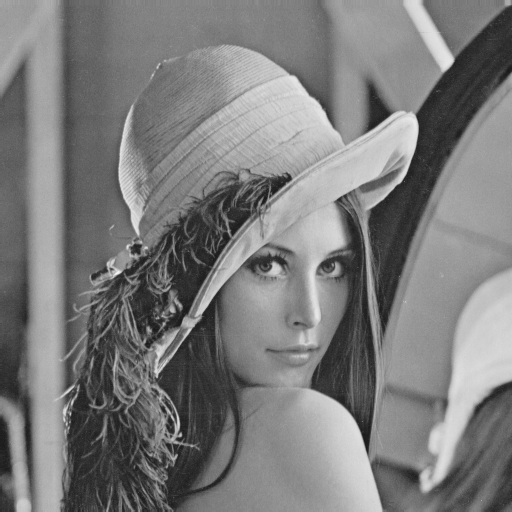
\includegraphics[scale=0.5]{img/Lena_L.png}
        \caption{Lena原图}
    \end{figure}

    \begin{figure}
        \center 
        \subfigure{
            \begin{minipage}[t]{0.3\linewidth}
                \centering
                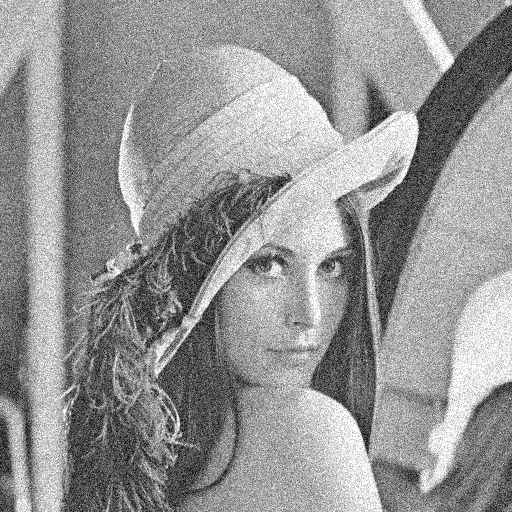
\includegraphics[width=1in]{img/Lena_no_gs_1.png}
                \caption{高斯噪声0.1}
            \end{minipage}
        }
        \subfigure{
            \begin{minipage}[t]{0.3\linewidth}
                \centering
                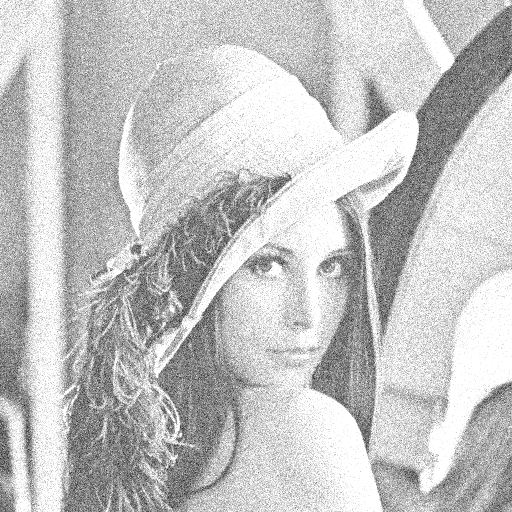
\includegraphics[width=1in]{img/Lena_no_gs_2.png}
                \caption{高斯噪声0.3}
            \end{minipage}
        }
        \subfigure{
            \begin{minipage}[t]{0.3\linewidth}
                \centering
                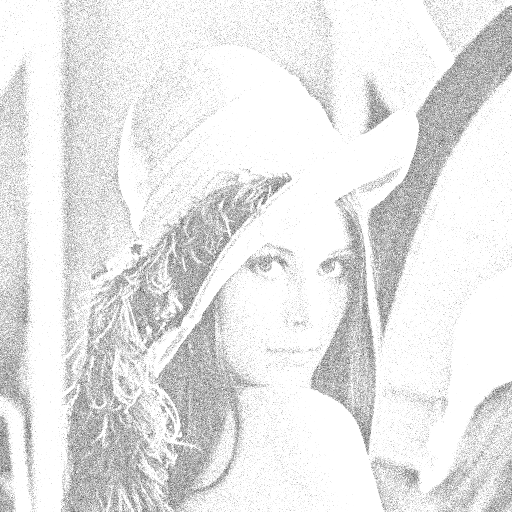
\includegraphics[width=1in]{img/Lena_no_gs_3.png}
                \caption{高斯噪声0.5}
            \end{minipage}
        }
        \subfigure{
            \begin{minipage}[t]{0.3\linewidth}
                \centering
                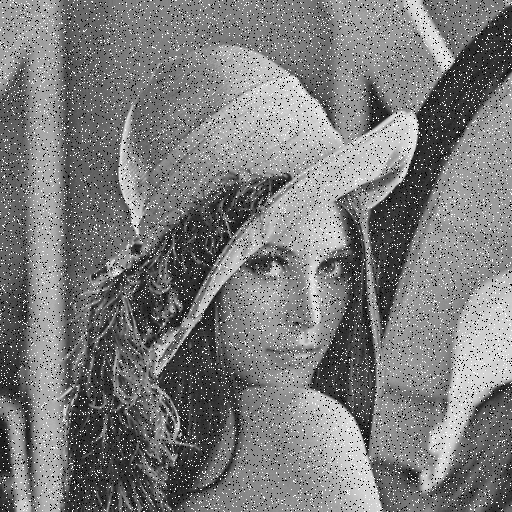
\includegraphics[width=1in]{img/Lena_no_sa&pe_1.png}
                \caption{椒盐噪声0.1}
            \end{minipage}
        }
        \subfigure{
            \begin{minipage}[t]{0.3\linewidth}
                \centering
                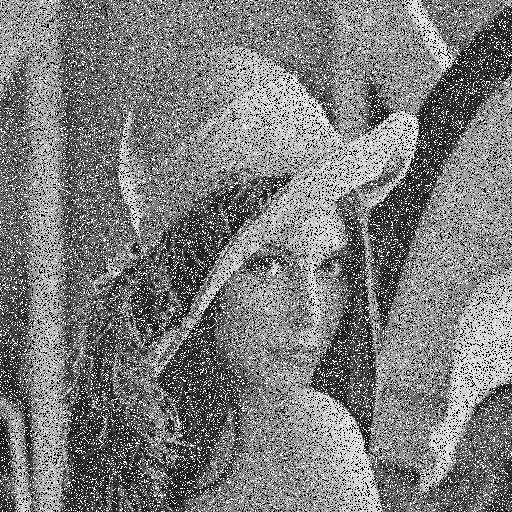
\includegraphics[width=1in]{img/Lena_no_sa&pe_2.png}
                \caption{椒盐噪声0.3}
            \end{minipage}
        }
        \subfigure{
            \begin{minipage}[t]{0.3\linewidth}
                \centering
                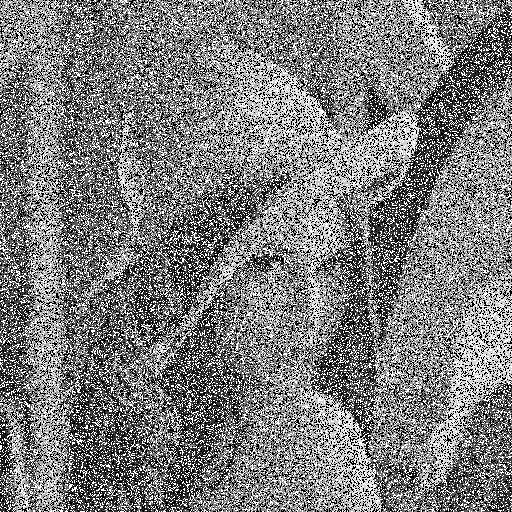
\includegraphics[width=1in]{img/Lena_no_sa&pe_3.png}
                \caption{椒盐噪声0.5}
            \end{minipage}
        }
    \end{figure}\par

    \begin{itemize}
        \item 均值滤波器
        \begin{itemize}
            \item 算数均值滤波器
            \item 几何均值滤波器
            \item 谐波均值滤波器
            \item 逆谐波均值滤波器
            \item 修正的Alpha均值滤波器
        \end{itemize}
        \item 中值滤\item 算数均值滤波器波器
        \item 最小值滤波器
        \item 最大值滤波器
    \end{itemize}\par

    \begin{figure}
        \center 
        \subfigure{
            \begin{minipage}[t]{0.45\linewidth}
                \centering
                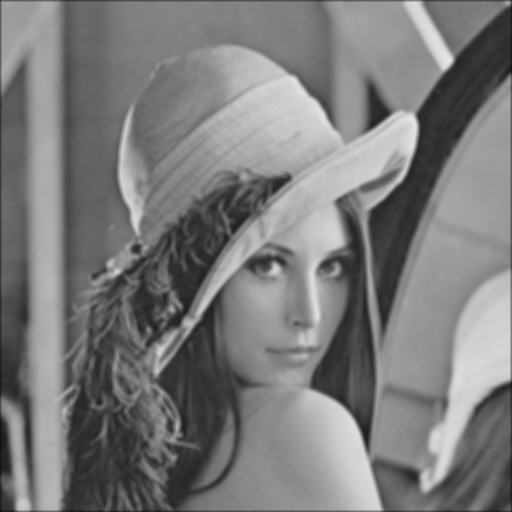
\includegraphics[width=1in]{img/res01.png}
                \caption{均值滤波器}
            \end{minipage}
        }
        \subfigure{
            \begin{minipage}[t]{0.45\linewidth}
                \centering
                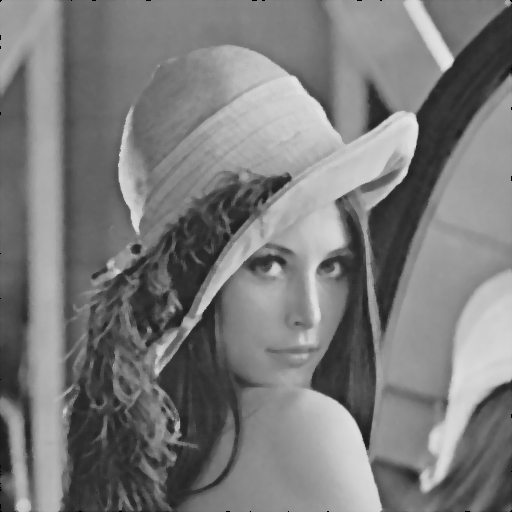
\includegraphics[width=1in]{img/res02.png}
                \caption{中值滤波器}
            \end{minipage}
        }
        \subfigure{
            \begin{minipage}[t]{0.45\linewidth}
                \centering
                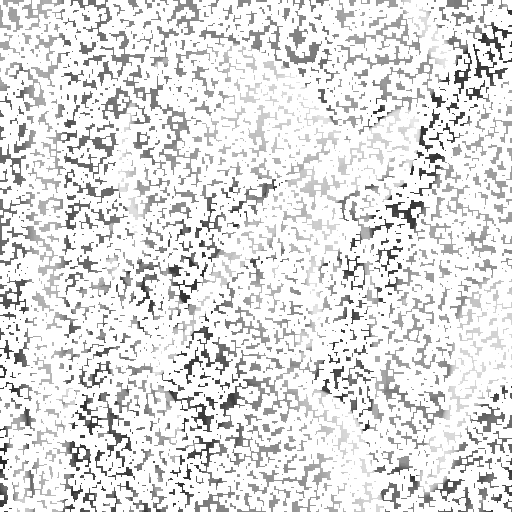
\includegraphics[width=1in]{img/res03.png}
                \caption{最小值滤波器}
            \end{minipage}
        }
        \subfigure{
            \begin{minipage}[t]{0.45\linewidth}
                \centering
                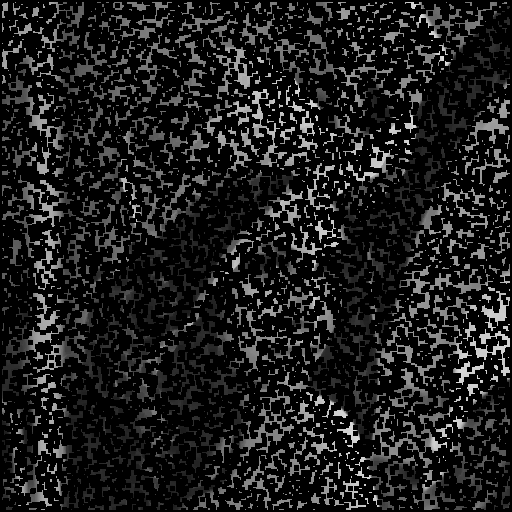
\includegraphics[width=1in]{img/res04.png}
                \caption{最大值滤波器}
            \end{minipage}
        }
        \caption{对椒盐噪声影响的图像进行滤波}
    \end{figure}\par


    算法的概述:

        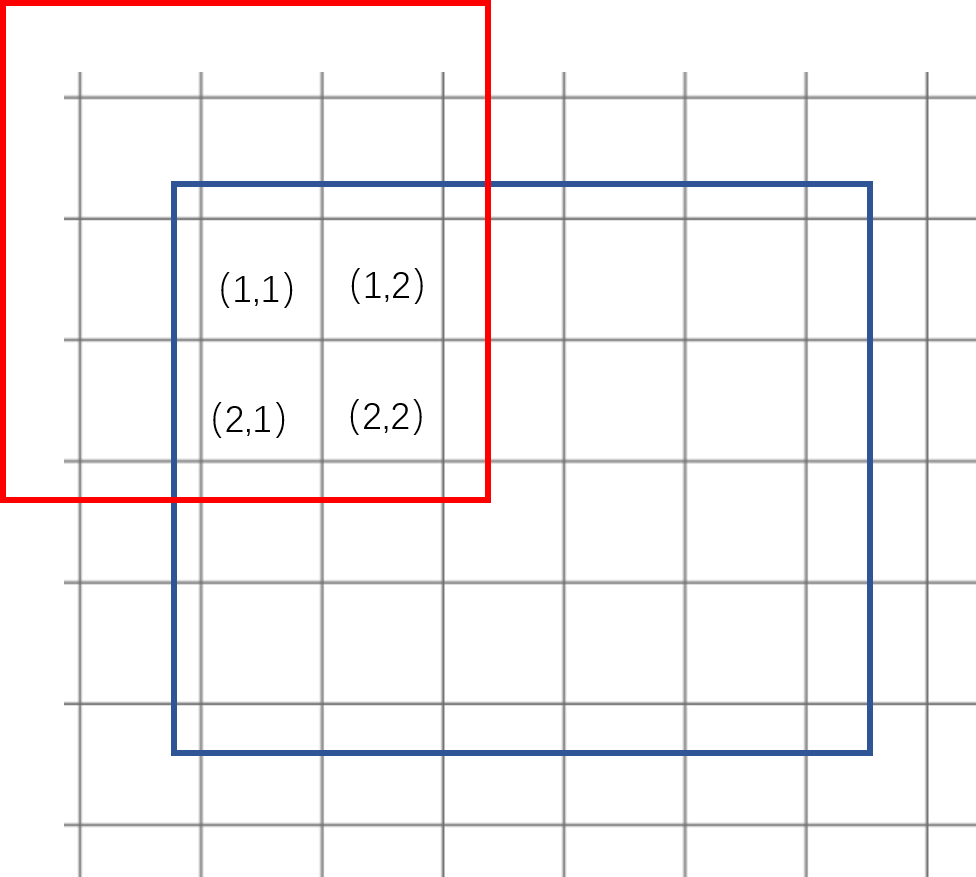
\includegraphics[width=0.8\linewidth]{img/ref1.png}   
    
        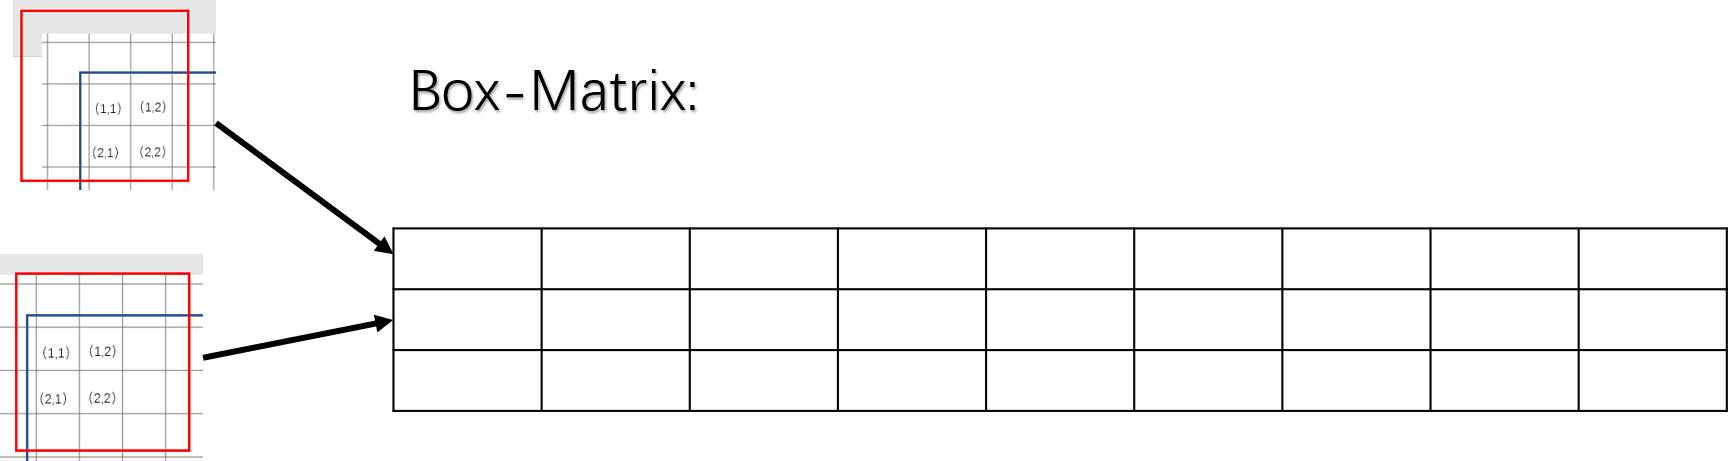
\includegraphics[width=0.8\linewidth]{img/ref2.png}

    红色的方框代表了滤波盒选择的像素,蓝色的方框内的是原图像的像
    素点矩阵。首先将原图像外扩一周,保证原图像边界像素的盒子,然
    后依次将盒中的像素对应到Box矩阵中,每一行存放的就是盒子里的
    所有像素。接下来对应的对盒子(也就是box矩阵的每一行做相应的
处理)。我们认为盒子里的像素(外扩的矩阵)的位置是 $ g(x,y) $
    处理后的矩阵的像素为$f(x,y)$,外扩矩阵:$S(x,y)$

    首先是算数均值滤波器,就是将盒子里的像素求和取平均:\\

    \begin{align}
        f(x,y) = \frac{1}{n} \sum_{(x,y)\in S(x,y)} g(x,y)
    \end{align}
    对应于box矩阵中一行的求和平均
    
    代码实现:
    \begin{lstlisting}
        out1(i,j) = floor(sum(box((i-1)*sizeImg(1)+j,:))/9);
    \end{lstlisting}
    效果对比:
    \begin{figure}[]
        \centering
        \subfigure{
            \begin{minipage}[t]{0.45\linewidth}
                \centering
                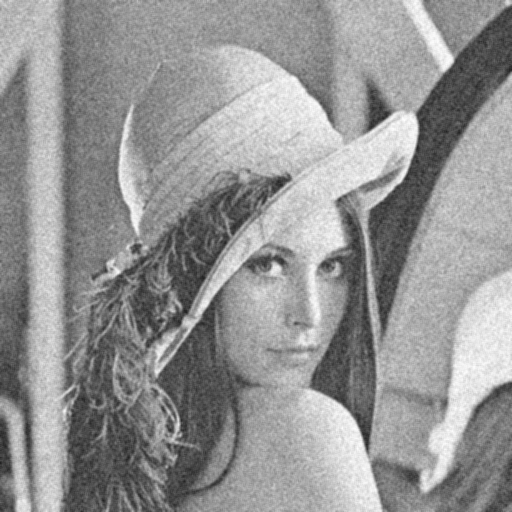
\includegraphics[width=2in]{img/althmMean_gs.png}
                \caption{对高斯噪声处理}
            \end{minipage}
        }
        \subfigure{
            \begin{minipage}[t]{0.45\linewidth}
                \centering
                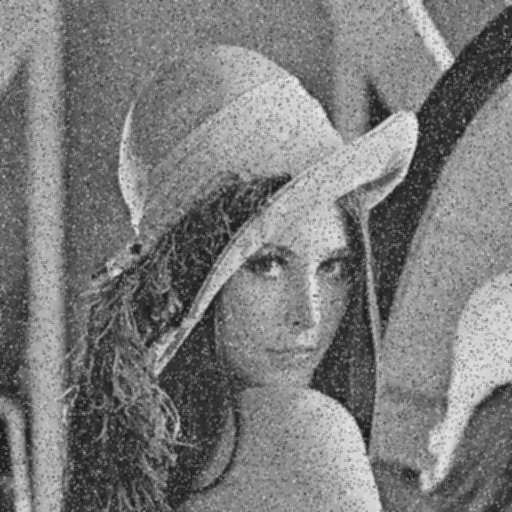
\includegraphics[width=2in]{img/althmMean_sp.png}
                \caption{对椒盐噪声处理}
            \end{minipage}
        }
        \caption{算数均值滤波器的处理效果}
    \end{figure}

    几何均值滤波器就是每一行的几何均值:
    \begin{align}
        f(x,y) = {\prod_{(x,y)\in S(x,y)} g(x,y)} ^{\frac{1}{n}}
    \end{align}
    
    效果对比:
    \begin{figure}[]
        \centering
        \subfigure{
            \begin{minipage}[t]{0.45\linewidth}
                \centering
                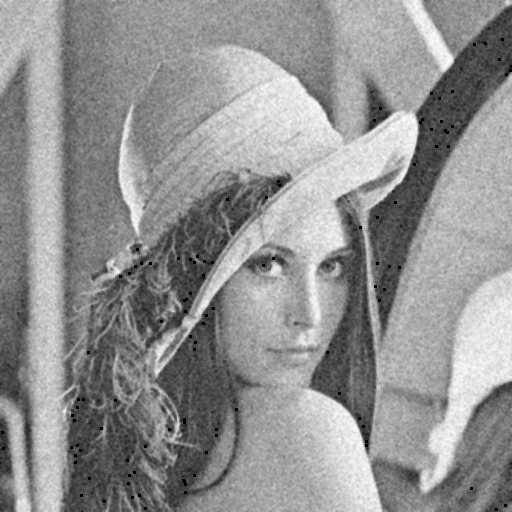
\includegraphics[width=2in]{img/geomMean_gs.png}
                \caption{对高斯噪声处理}
            \end{minipage}
        }
        \subfigure{
            \begin{minipage}[t]{0.45\linewidth}
                \centering
                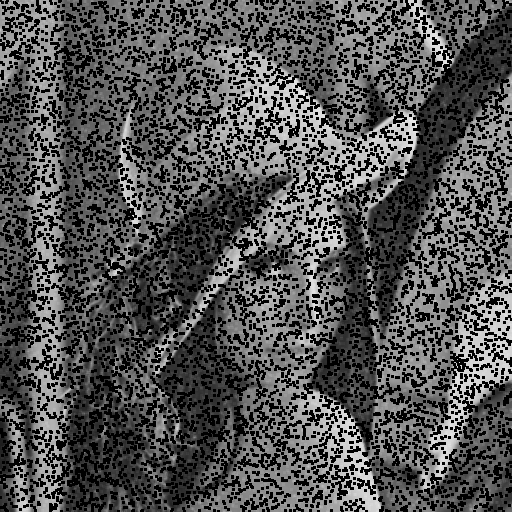
\includegraphics[width=2in]{img/geomMean_sp.png}
                \caption{对椒盐噪声处理}
            \end{minipage}
        }
        \caption{几何均值滤波器的处理效果}
    \end{figure}

    谐波均值滤波器:
    \begin{align}
        f(x,y) = \frac{n}{\sum \frac{1}{g(x,y)}} 
    \end{align}

    效果对比:
    \begin{figure}[]
        \centering
        \subfigure{
            \begin{minipage}[t]{0.45\linewidth}
                \centering
                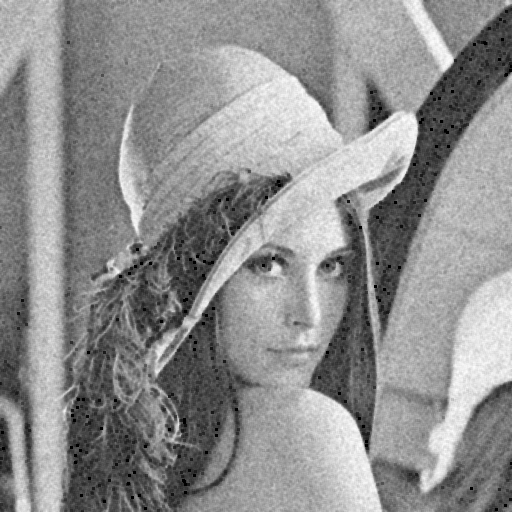
\includegraphics[width=2in]{img/harmMean_gs.png}
                \caption{对高斯噪声处理}
            \end{minipage}
        }
        \subfigure{
            \begin{minipage}[t]{0.45\linewidth}
                \centering
                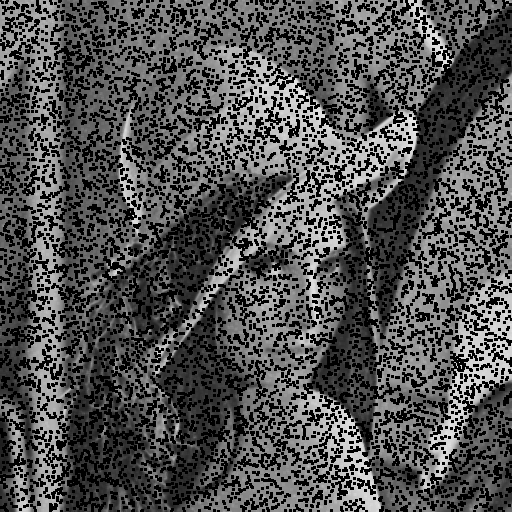
\includegraphics[width=2in]{img/harmMean_sp.png}
                \caption{对椒盐噪声处理}
            \end{minipage}
        }
        \caption{谐波均值滤波器的处理效果}
    \end{figure}

    逆谐波均值滤波器:
    \begin{align}
        f(x,y) = \frac{\sum {g(x,y)} ^{Q+1}}{\sum {g(x,y)} ^{Q}} 
    \end{align}

    效果对比:
    \begin{figure}[]
        \centering
        \subfigure{
            \begin{minipage}[t]{0.45\linewidth}
                \centering
                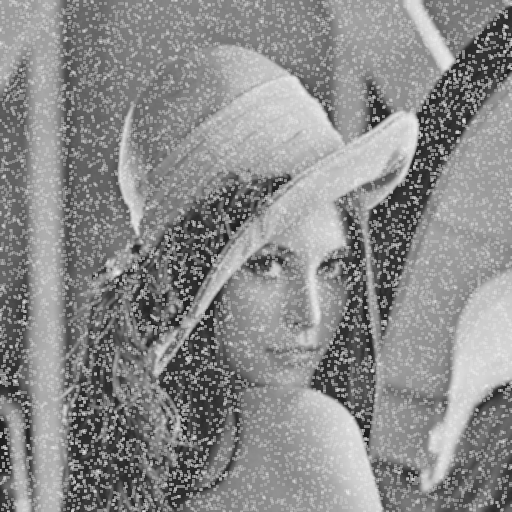
\includegraphics[width=2in]{img/contrHarmMean_sp_po.png}
                \caption{参数为正,消除焦噪声}
            \end{minipage}
        }
        \subfigure{
            \begin{minipage}[t]{0.45\linewidth}
                \centering
                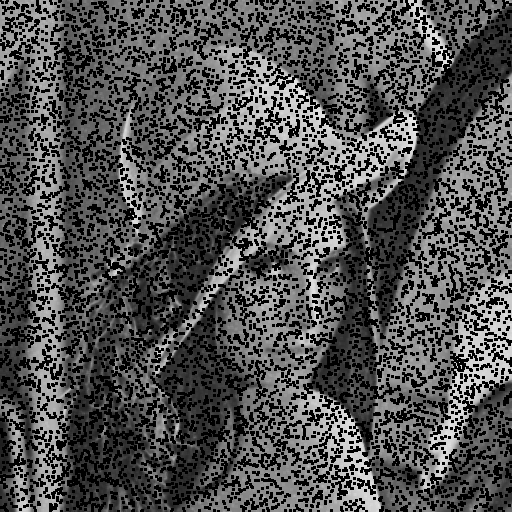
\includegraphics[width=2in]{img/contrHarmMean_sp_ne.png}
                \caption{参数-1,等于几何均值}
            \end{minipage}
        }
        \subfigure{
            \begin{minipage}[t]{0.45\linewidth}
                \centering
                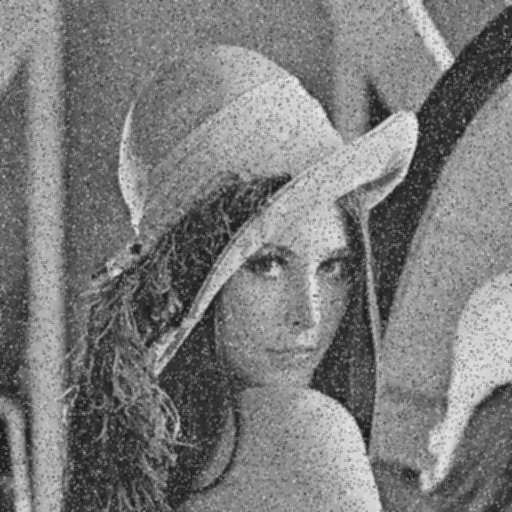
\includegraphics[width=2in]{img/contrHarmMean_sp_ze.png}
                \caption{参数为0,等于算数均值}
            \end{minipage}
        }
        \caption{逆谐波均值滤波器的处理效果}
    \end{figure}

    中值滤波器就是寻找盒中的中值:

    代码如下:
    \begin{lstlisting}
        out1(i,j) = median(box((i-1)*sizeImg(1)+j,:));
    \end{lstlisting}

    最大值,最小值,中点同理,具体代码详见maxFliter.m minFliter.m 和 midFliter.m

    效果对比:
    \begin{figure}[]
        \centering
        \subfigure{
            \begin{minipage}[t]{0.45\linewidth}
                \centering
                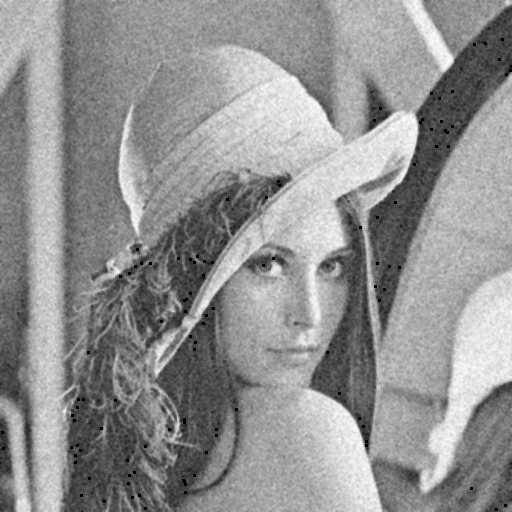
\includegraphics[width=2in]{img/geomMean_gs.png}
                \caption{对高斯噪声处理}
            \end{minipage}
        }
        \subfigure{
            \begin{minipage}[t]{0.45\linewidth}
                \centering
                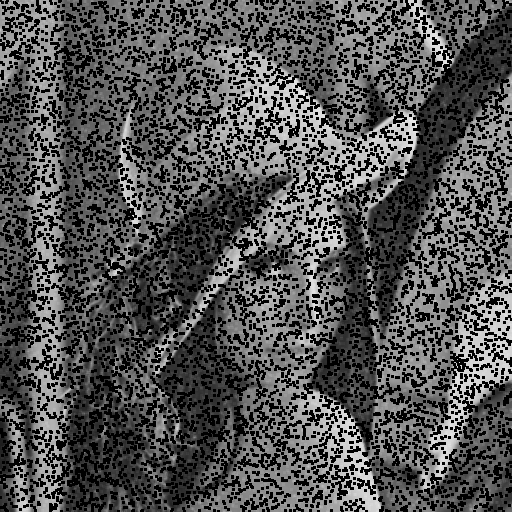
\includegraphics[width=2in]{img/geomMean_sp.png}
                \caption{对椒盐噪声处理}
            \end{minipage}
        }
        \caption{几何均值滤波器的处理效果}
    \end{figure}

    谐波均值滤波器:
    \begin{align}
        f(x,y) = \frac{n}{\sum \frac{1}{g(x,y)}} 
    \end{align}

    效果对比:
    \begin{figure}[]
        \centering
        \subfigure{
            \begin{minipage}[t]{0.45\linewidth}
                \centering
                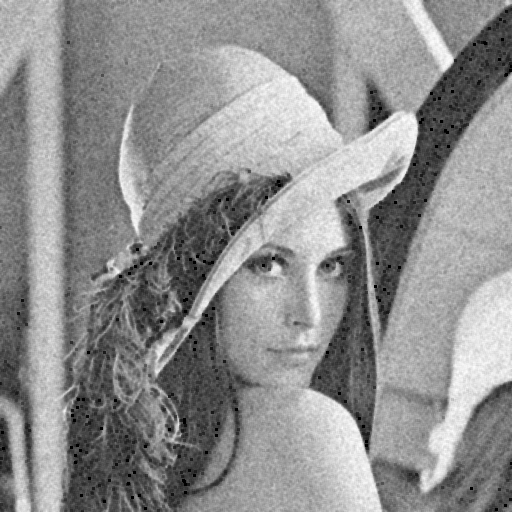
\includegraphics[width=2in]{img/harmMean_gs.png}
                \caption{对高斯噪声处理}
            \end{minipage}
        }
        \subfigure{
            \begin{minipage}[t]{0.45\linewidth}
                \centering
                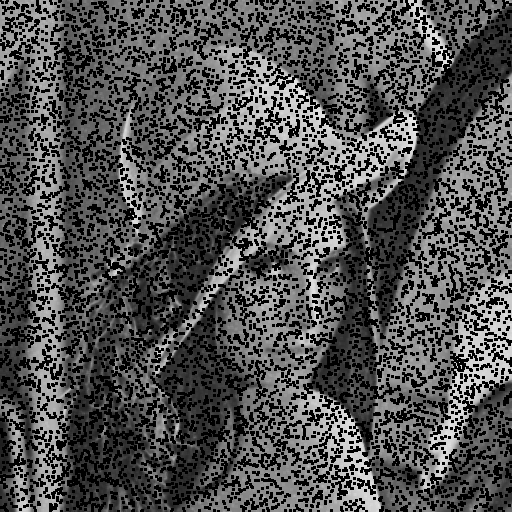
\includegraphics[width=2in]{img/harmMean_sp.png}
                \caption{对椒盐噪声处理}
            \end{minipage}
        }
        \caption{谐波均值滤波器的处理效果}
    \end{figure}

    逆谐波均值滤波器:
    \begin{align}
        f(x,y) = \frac{\sum {g(x,y)} ^{Q+1}}{\sum {g(x,y)} ^{Q}} 
    \end{align}

    效果对比:
    \begin{figure}[]
        \centering
        \subfigure{
            \begin{minipage}[t]{0.45\linewidth}
                \centering
                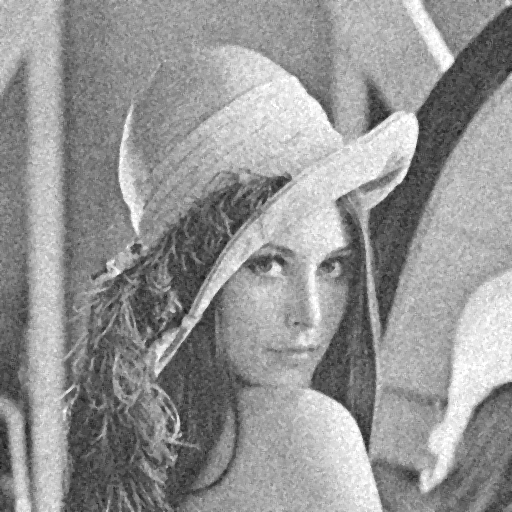
\includegraphics[width=2in]{img/meaidan_gs.png}
                \caption{中值滤波,高斯噪声}
            \end{minipage}
        }
        \subfigure{
            \begin{minipage}[t]{0.45\linewidth}
                \centering
                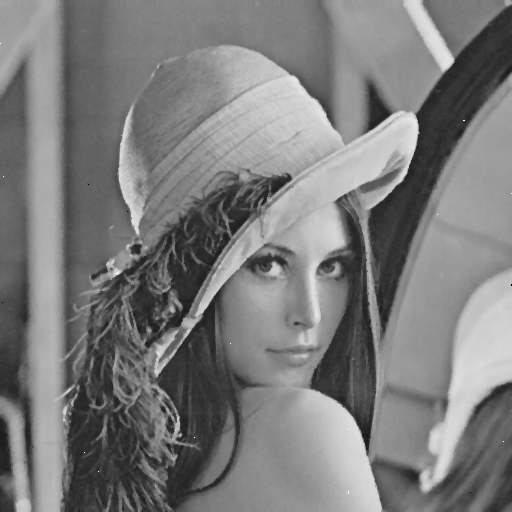
\includegraphics[width=2in]{img/meaidan_sp.png}
                \caption{中值滤波,椒盐噪声}
            \end{minipage}
        }
        \caption{中值滤波器的处理效果}
    \end{figure}

    \begin{figure}[]
        \centering
        \subfigure{
            \begin{minipage}[t]{0.45\linewidth}
                \centering
                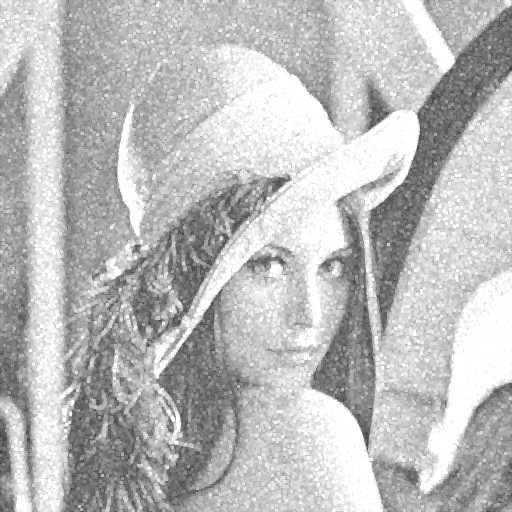
\includegraphics[width=2in]{img/maxFliter_gs.png}
                \caption{最大值滤波,高斯噪声}
            \end{minipage}
        }
        \subfigure{
            \begin{minipage}[t]{0.45\linewidth}
                \centering
                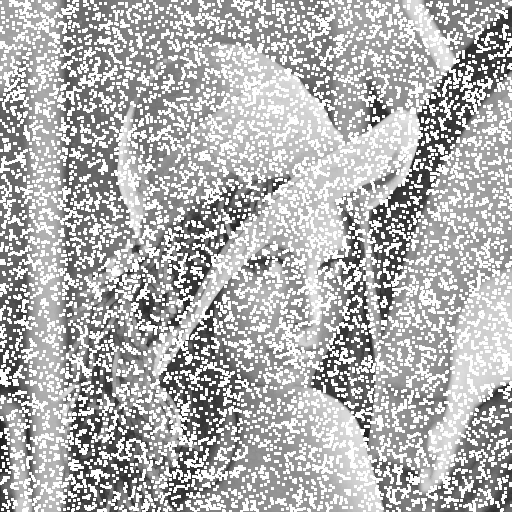
\includegraphics[width=2in]{img/maxFliter_sp.png}
                \caption{最大滤波,椒盐噪声}
            \end{minipage}
        }
        \caption{最大值滤波器的处理效果}
    \end{figure}
    \begin{figure}[]
        \centering
        \subfigure{
            \begin{minipage}[t]{0.45\linewidth}
                \centering
                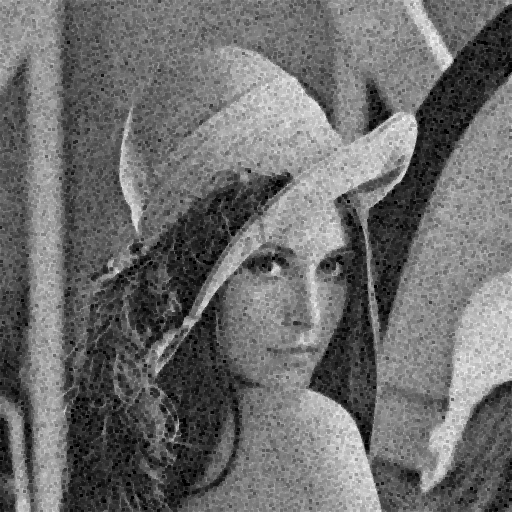
\includegraphics[width=2in]{img/minFliter_gs.png}
                \caption{最小值滤波,高斯噪声}
            \end{minipage}
        }
        \subfigure{
            \begin{minipage}[t]{0.45\linewidth}
                \centering
                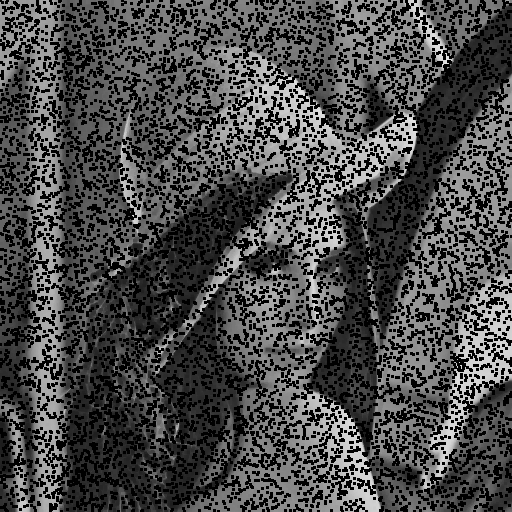
\includegraphics[width=2in]{img/minFliter_sp.png}
                \caption{最小值滤波,椒盐噪声}
            \end{minipage}
        }
        \caption{最小值滤波器的处理效果}
    \end{figure}
    

    修正的 $\alpha $均值滤波器,是去掉盒中的 n 个最大,最小值的算数均值滤波器

    
    \begin{figure}[]
        \centering
        \subfigure{
            \begin{minipage}[t]{0.45\linewidth}
                \centering
                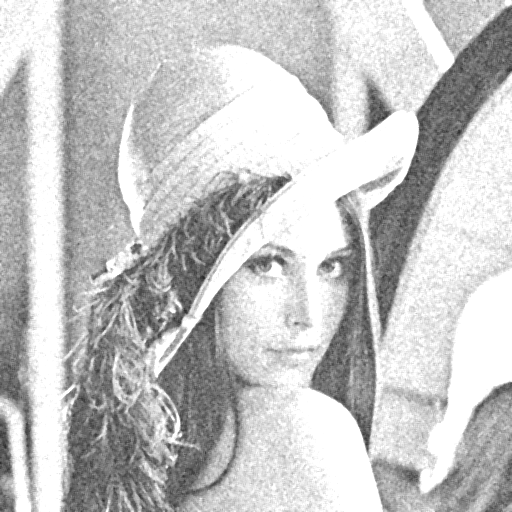
\includegraphics[width=2in]{img/modf_AlphaFliter_gs.png}
                \caption{$\alpha$均值滤波,高斯噪声}
            \end{minipage}
        }
        \subfigure{
            \begin{minipage}[t]{0.45\linewidth}
                \centering
                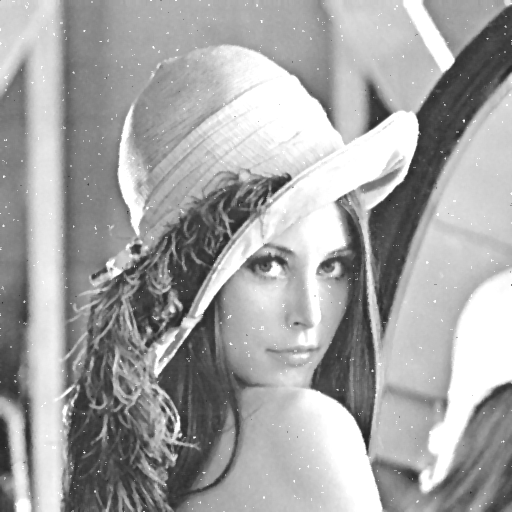
\includegraphics[width=2in]{img/modf_AlphaFliter_sp.png}
                \caption{$\alpha$均值滤波,椒盐噪声}
            \end{minipage}
        }
        \caption{最大值滤波器的处理效果}
    \end{figure}
    $\alpha$均值滤波器的阈值取到大到舍弃的最大最小值为滤波盒的一半时,就变成
    了中值滤波。

\end{document}out1(i,j) = median(box((i-1)*sizeImg(1)+j,:));
